\section{Nachhaltigkeit}

Im Sinne einer ressourcenschonenden Entwicklung, angelehnt an das 3R-Prinzip (Reduce, Reuse, Recycle) sowie das 12. Ziel für nachhaltige Entwicklung der Vereinten Nationen („Nachhaltige Konsum- und Produktionsmuster sicherstellen“), wurde die Wiederverwendbarkeit von Bauteilen gezielt berücksichtigt. Die Grundplatte des Prototyps aus PREN1 wurde so konstruiert, dass sie modular erweiterbar ist. Zusätzliche Bohrungen und Nuten konnten während der Entwicklung fortlaufend eingebracht werden, ohne dass eine neue Platte gefertigt werden musste. Die Nachbearbeitung mittels Laserschneidmaschine verlief dabei ohne technische Probleme. Dadurch konnte der Materialeinsatz auf eine einzige Grundplatte beschränkt und die Entstehung von Abfall minimiert werden. Eine Übersicht der verschiedenen Bearbeitungszustände ist in Abbildung \ref{fig: Weiterentwicklung der Grundplatte} dargestellt.


\begin{figure}[H] % oder [htbp]
    \centering
    \begin{subfigure}[b]{0.45\textwidth}
        \centering
        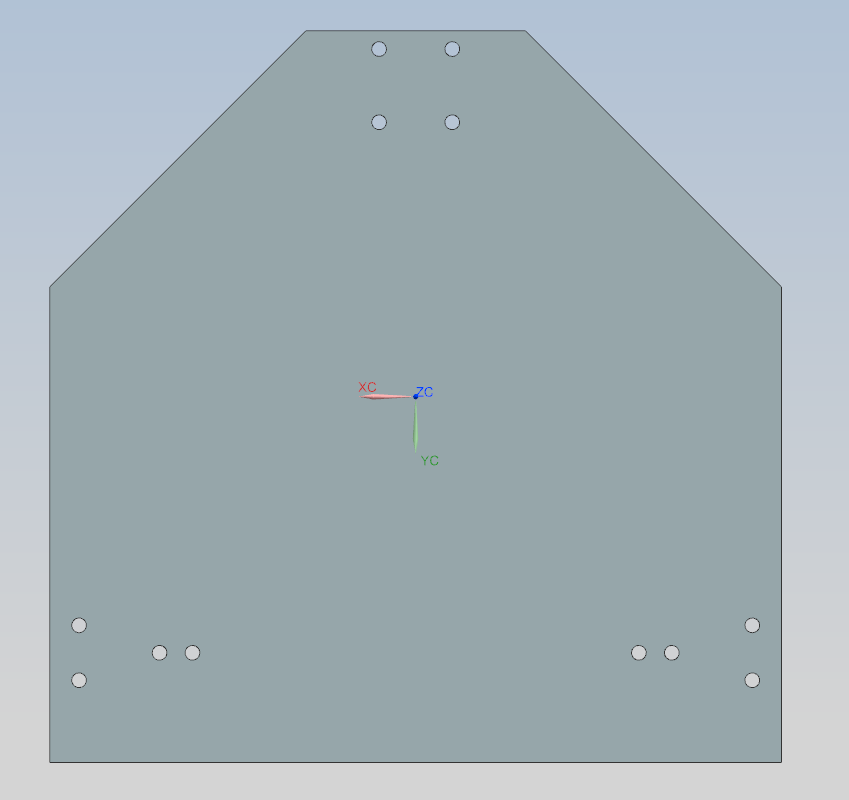
\includegraphics[width=\linewidth]{assets/MT/Grundplatte_V0.png}
        \caption{Grundplatte V0}
    \end{subfigure}
    \hfill
    \begin{subfigure}[b]{0.45\textwidth}
        \centering
        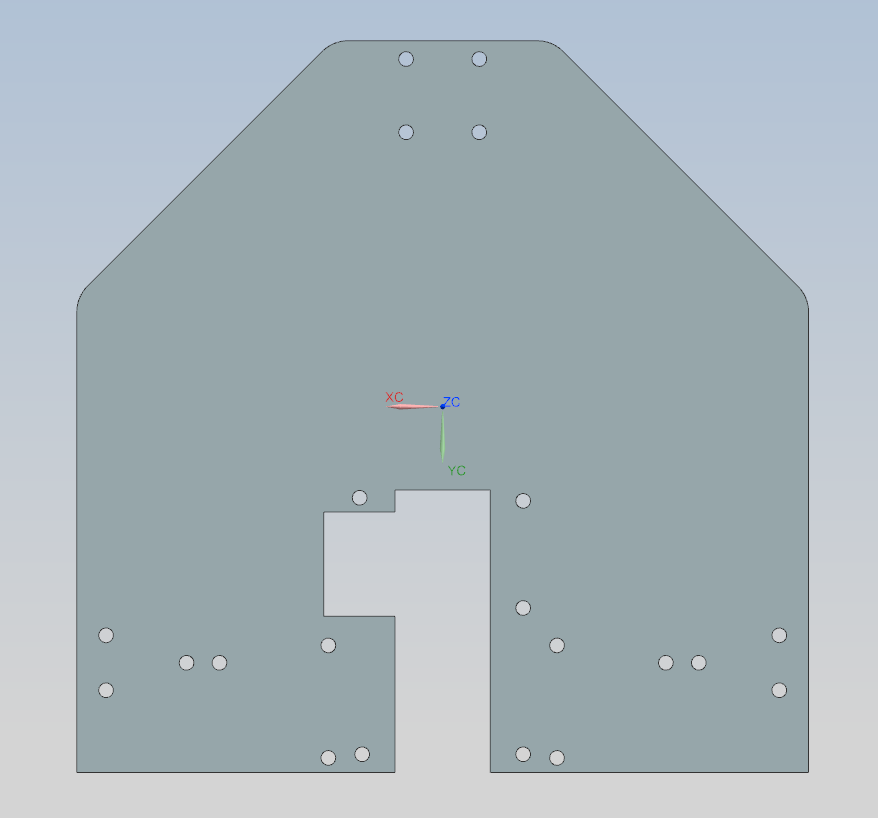
\includegraphics[width=\linewidth]{assets/MT/Grundplatte_V1.png}
        \caption{Grundplatte V1}
    \end{subfigure}

    \vspace{0.5cm}

    \begin{subfigure}[b]{0.45\textwidth}
        \centering
        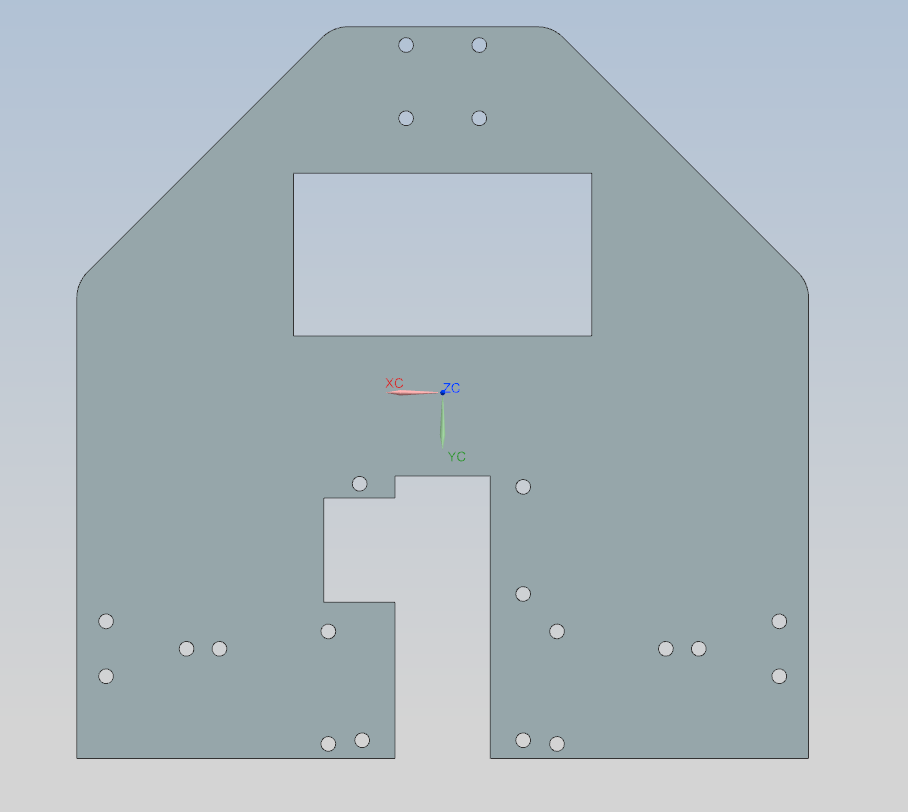
\includegraphics[width=\linewidth]{assets/MT/Grundplatte_V2.png}
        \caption{Grundplatte V2}
    \end{subfigure}
    \hfill
    \begin{subfigure}[b]{0.45\textwidth}
        \centering
        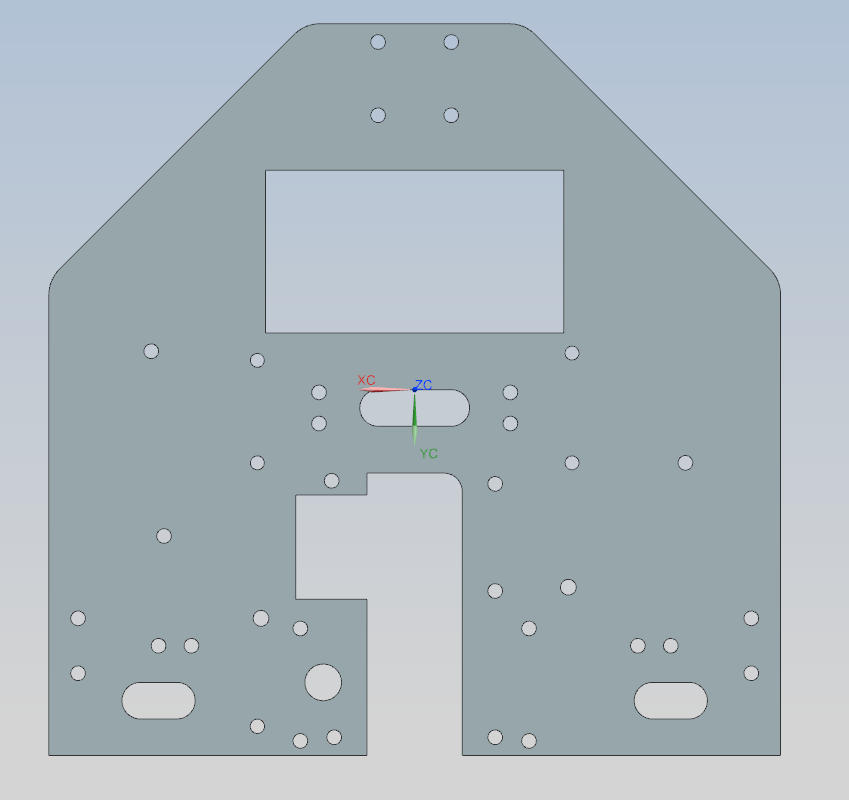
\includegraphics[width=\linewidth]{assets/MT/Grundplatte_V3.png}
        \caption{Grundplatte V3}
    \end{subfigure}
    \caption{Weiterentwicklung der Grundplatte}
    \label{fig: Weiterentwicklung der Grundplatte}
\end{figure}

\subsection{Oekobilanz}

\subsubsection{Material}

Was gibt es alles und wie viel davon?
\subsubsection{Entsorgung und Rezyklierbarkeit}
Was ist recyclebar? ...


3 Mengemaessig meiste (gewicht?)

3 schlechteste

min 2 Seiten